\documentclass[tikz,border=8pt]{standalone}
\usepackage{tikz}
\usepackage{xcolor}
\usepackage{amsmath}
\usepackage{amsfonts, amssymb}
\pagecolor{black}
\color{white}

% --- Define custom colors from palette ---
\definecolor{softblue}{HTML}{88a0dc}
\definecolor{deeppurple}{HTML}{CDBDF1}
\definecolor{plum}{HTML}{F5C5EB}
\definecolor{plumorig}{HTML}{7c4b73}
\definecolor{coralpink}{HTML}{ed968c}
\definecolor{deepred}{HTML}{ab3329}
\definecolor{orange}{HTML}{e78429}
\definecolor{gold}{HTML}{f9d14a}

\begin{document}
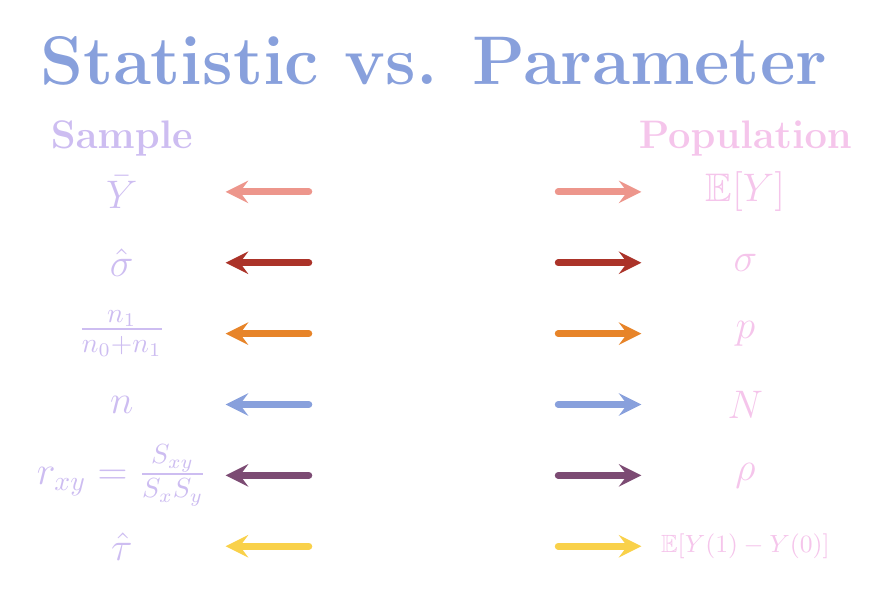
\begin{tikzpicture}[>=stealth, line cap=round, xscale=.33, yscale=.45]

% --- layout helpers ---
\def\L{-12.0}   % left column x
\def\C{0}      % center column x
\def\R{12.0}    % right column x

% --- title ---
\node[text=softblue, align=center, font=\bfseries\fontsize{34}{38}\selectfont]
  at (\C,9.7) {Statistic vs. Parameter};

% --- column headers ---
\node[font=\bfseries\Large, text=deeppurple] at (\L,7.5) {Sample};
\node[font=\bfseries\Large, text=plum] at (\R,7.5) {Population};

% --- a small macro for each row: y, label, left, right, arrowcolor 
\newcommand{\rowitem}[5]{%
  \node[font=\Large, text=white] at (\C,#1) {#2};
  \node[font=\Large, text=deeppurple] at (\L,#1) {#3};
  \node[font=\Large, text=plum] at (\R,#1) {#4};
  \draw[#5,->,line width=2.5pt] (\C-4.8,#1) -- (\L+4,#1);
  \draw[#5,->,line width=2.5pt] (\C+4.8,#1) -- (\R-4,#1);
}

% --- rows (top to bottom) with color semantics ---
\rowitem{6.0}{mean}{$\bar{Y}$}{$\mathbb E[Y]$}{coralpink}
\rowitem{4.0}{std.\ dev.}{$\hat \sigma$}{$\sigma$}{deepred}
\rowitem{2.0}{proportion}{$\frac{n_1}{n_0 + n_1}$}{$p$}{orange}
\rowitem{0.0}{size}{$n$}{$N$}{softblue}
\rowitem{-2.0}{correlation}{$r_{xy} = \frac{S_{xy}}{S_x S_y}$}{$\rho$}{plumorig}
\rowitem{-4.0}{ATE}{$\hat{\tau}$}{\small $\mathbb E[Y(1) - Y(0)]$}{gold}

\end{tikzpicture}
\end{document}

